\chapter{REVISIÓN CRÍTICA DE LA LITERATURA}

Para desarrollar un sistema tecnológico se debe conocer qué existe actualmente en el mercado, tanto en hardware como en software. En este sentido, se buscará entre las distintas empresas qué servicios realizan para las granjas de jaula, qué robots utilizan y qué métodos utilizan relacionados la visión computacional. Seguidamente, con el fin de simular correctamente el sistema desarrollado, se debe identificar qué software de simulación es el mejor para crear ambientes parecidos. 

\section{Empresas que genera soluciones en acuicultura}
La tecnología para la acuicultura es desarrollado por empresas contratistas que ofrecen distintos servicios. Cada una tiene un método distinto de ofrecerlos, ya sea con distintos equipos integrados o robots submarinos que lo simplifican o complementan. De acuerdo al sondeo realizado (ver anexo A), los servicios para las redes son los siguientes:

\subsection{Inspección de redes y sistemas de amarre}
Empresas como Qysea, AKVA group \cite{AKVAgroup} o UCO utilizan robots submarinos ROV (Vehículo Operado Remotamente) capaces de navegar alrededor de las granjas. Los servicios implican un operador in-situ manejando el ROV. Dentro de esta inspección, algunas empresas como Deep Trekker \cite{DeepTrekker}, Blue-eye robotics han desarrollado algoritmos de reconocimiento de huecos. Aún más, con sus ROVs pueden parchar tales huecos de manera rápida y simple. Una desventaja de estos servicios es que no realizan operaciones ni análisis autónomas, es decir, no utilizan herramientas de navegación autónoma o visión computacional respectivamente. 

\begin{figure} [!h]
    \begin{center}
    \begin{tabular}{ccc}
    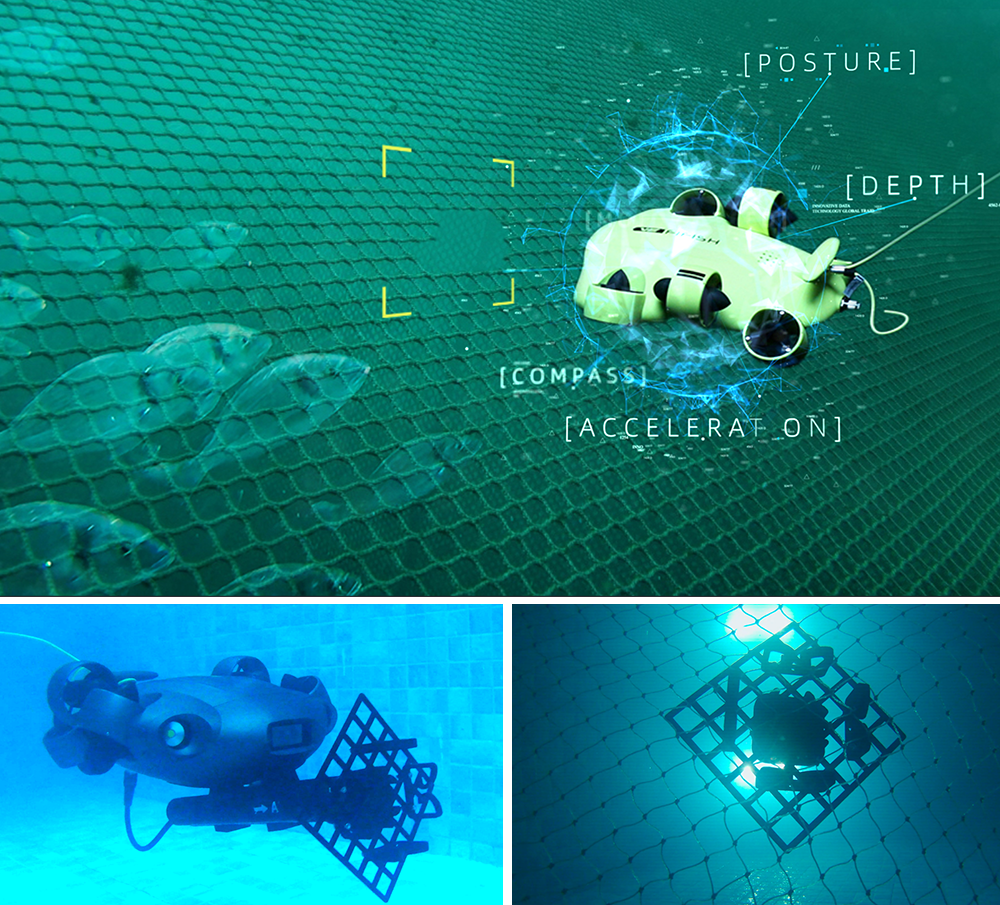
\includegraphics[height=3cm]{images/Qysea_1} &
    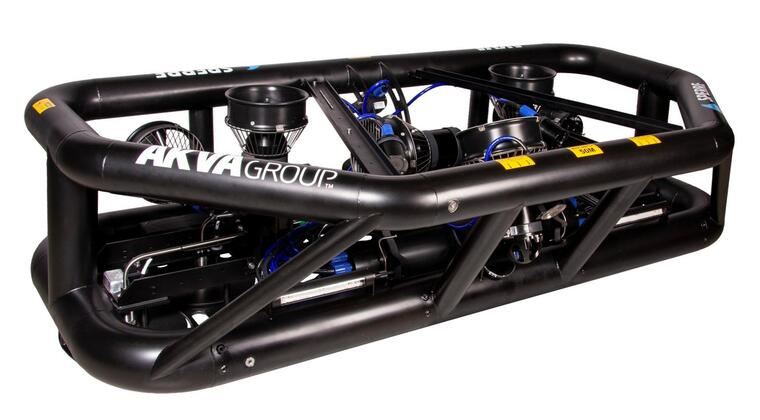
\includegraphics[height=2cm]{images/AKVA_1} &
    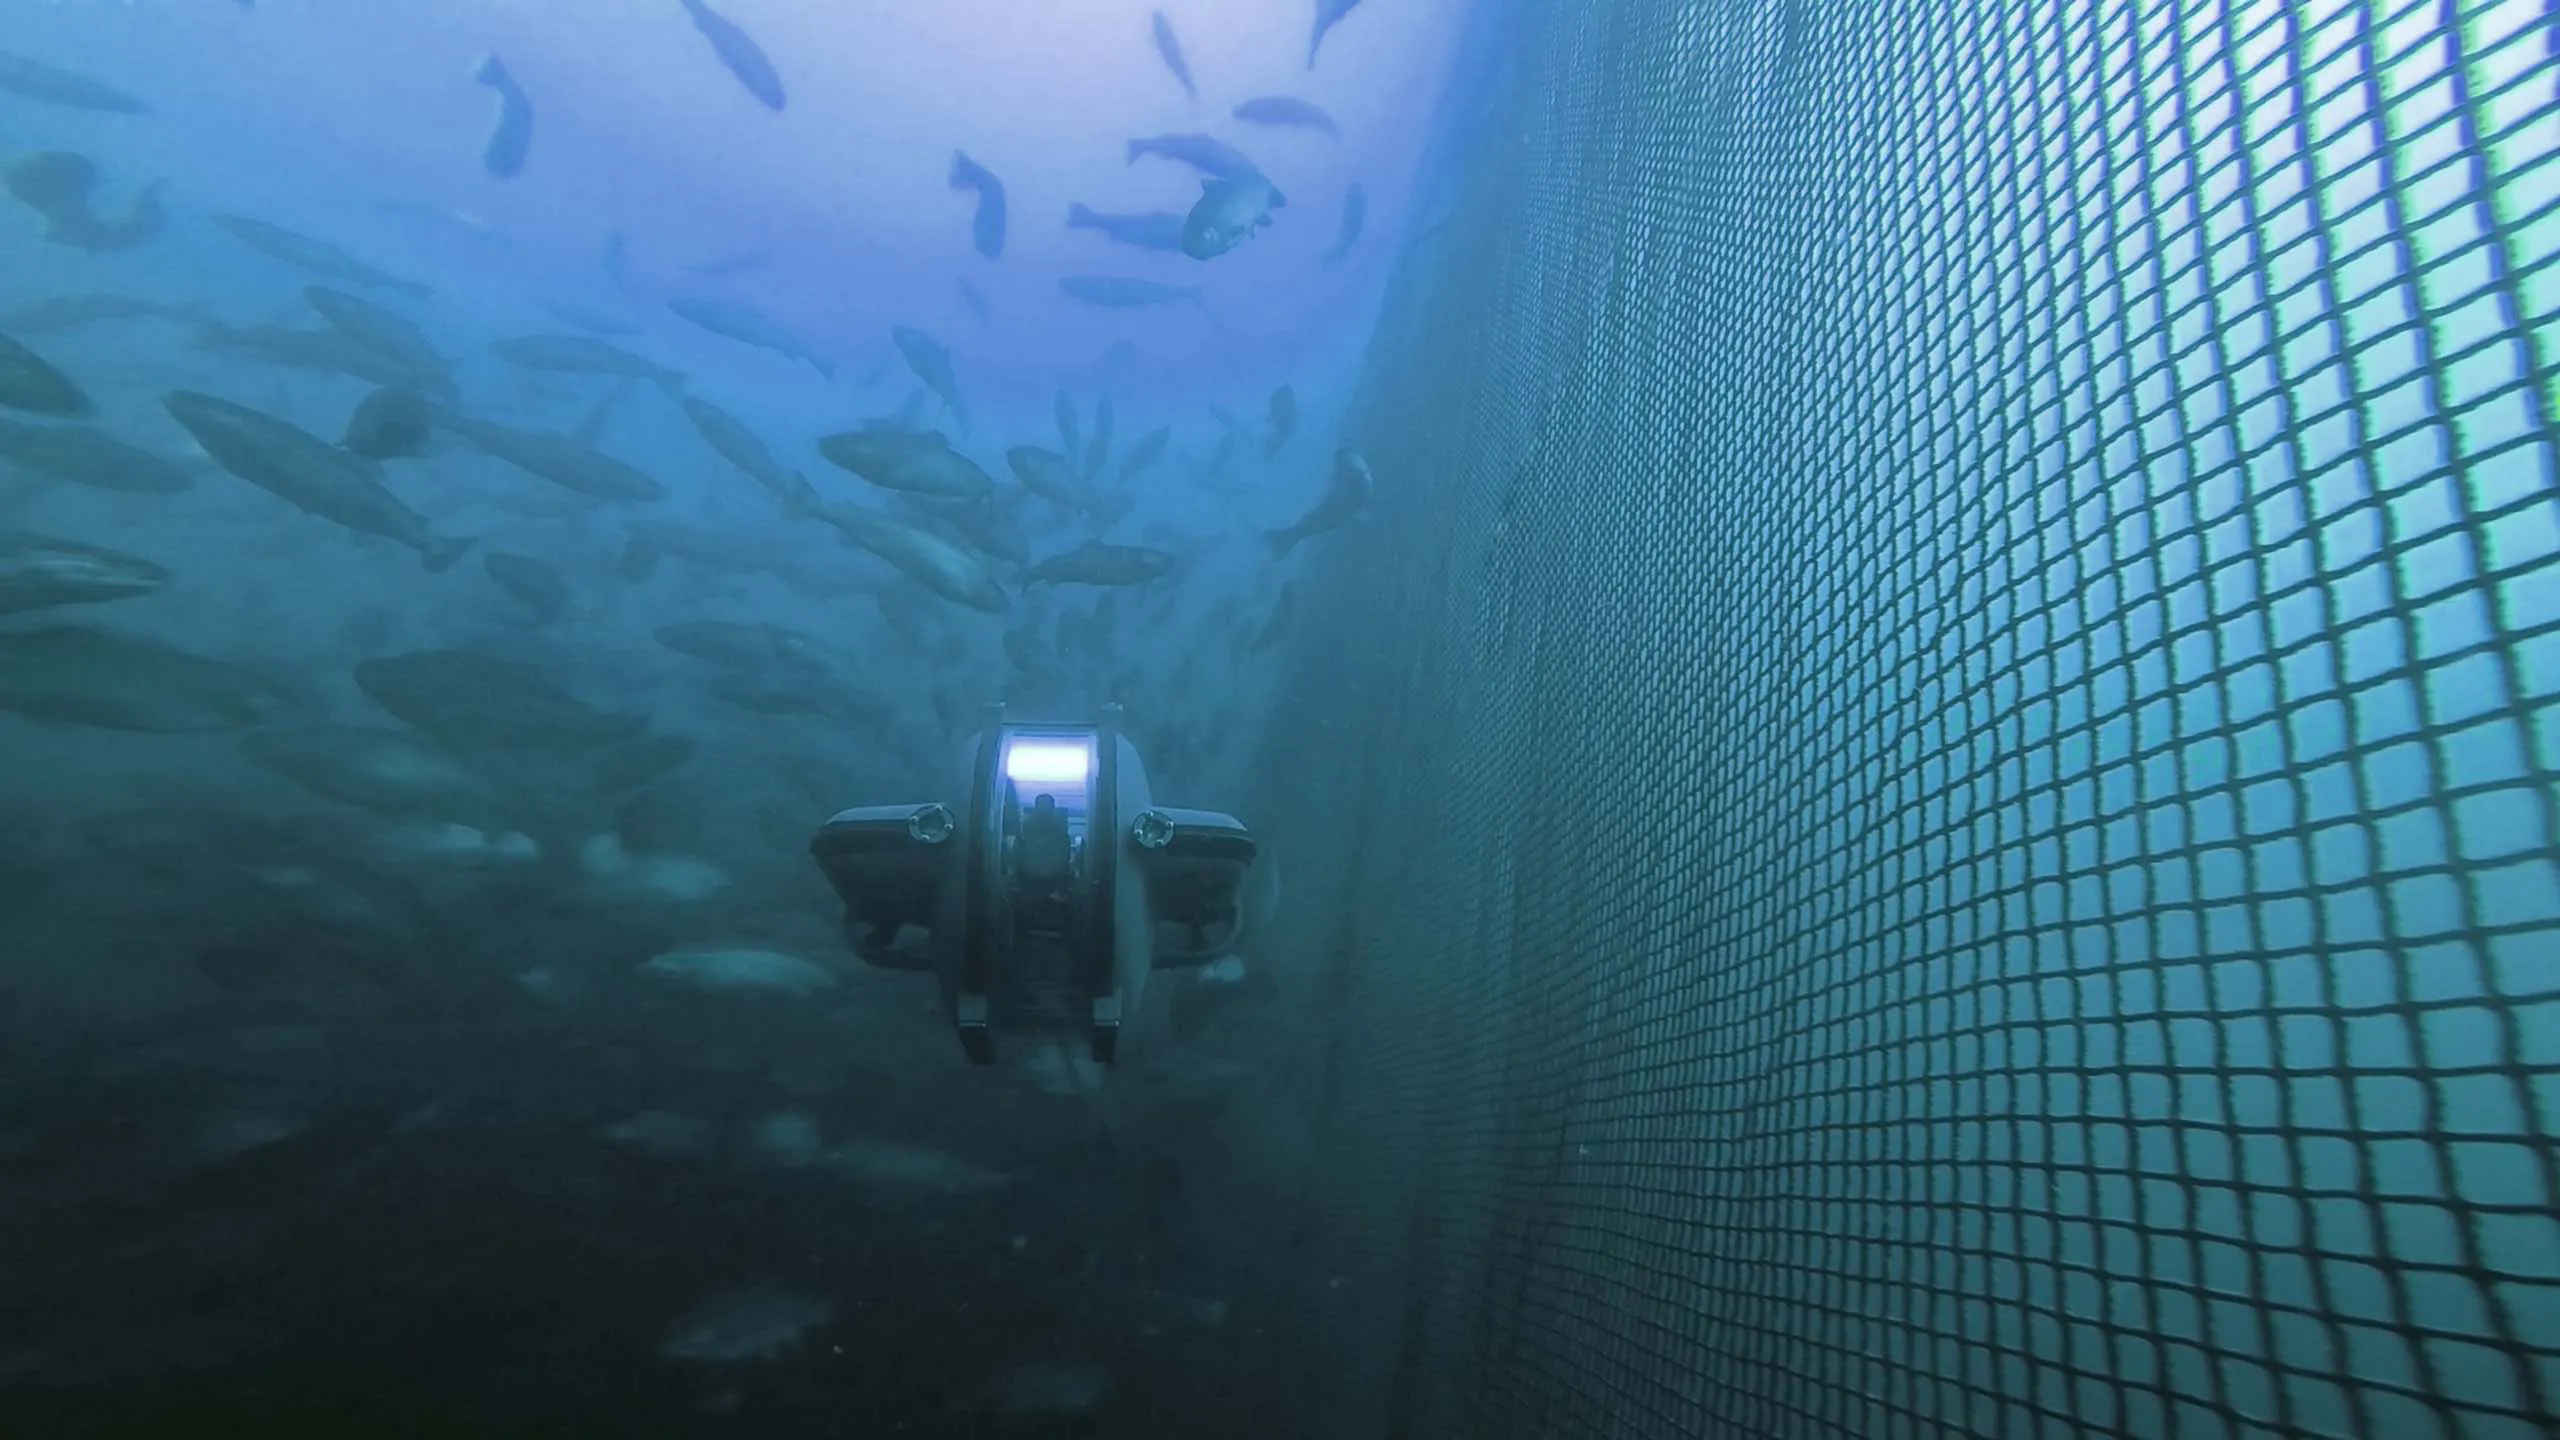
\includegraphics[height=3cm]{images/Deep_1} \\
    (a) & (b) & (c)
    \end{tabular}
    \caption{\label{fig:empresas_manual}(a) ROV de Qysea para reparación de huecos. (b) Robot de AKVA para limpieza de redes. (c) ROV de Deep Trekker para inspección manual de redes.}
    \end{center}
\end{figure}


En contraste con las empresas mencionadas, InnovaSea \cite{InnovaSea} ofrece un sistema completo conformado por distintos equipos entre las granjas que miden parámetros del agua, nivel de alimentación, comportamiento y salud del pescado. Posee un dispositivo entre las conexiones cada granja, controlando el sistema de amarre. Sin embargo, no ofrece una solución para la inspección de redes. Cabe resaltar que tampoco utiliza ROVs, mas sí dispositivos que, para otros parámetros, realiza mediciones de forma estática. Para análisis de estas mediciones, a comparación de las empresas anteriormente mencionadas, sí utilizan herramientas de visión computacional para obtener la biomasa del pescado, control de alimentación, entre otros. 

\begin{figure} [!h]
    \begin{center}
    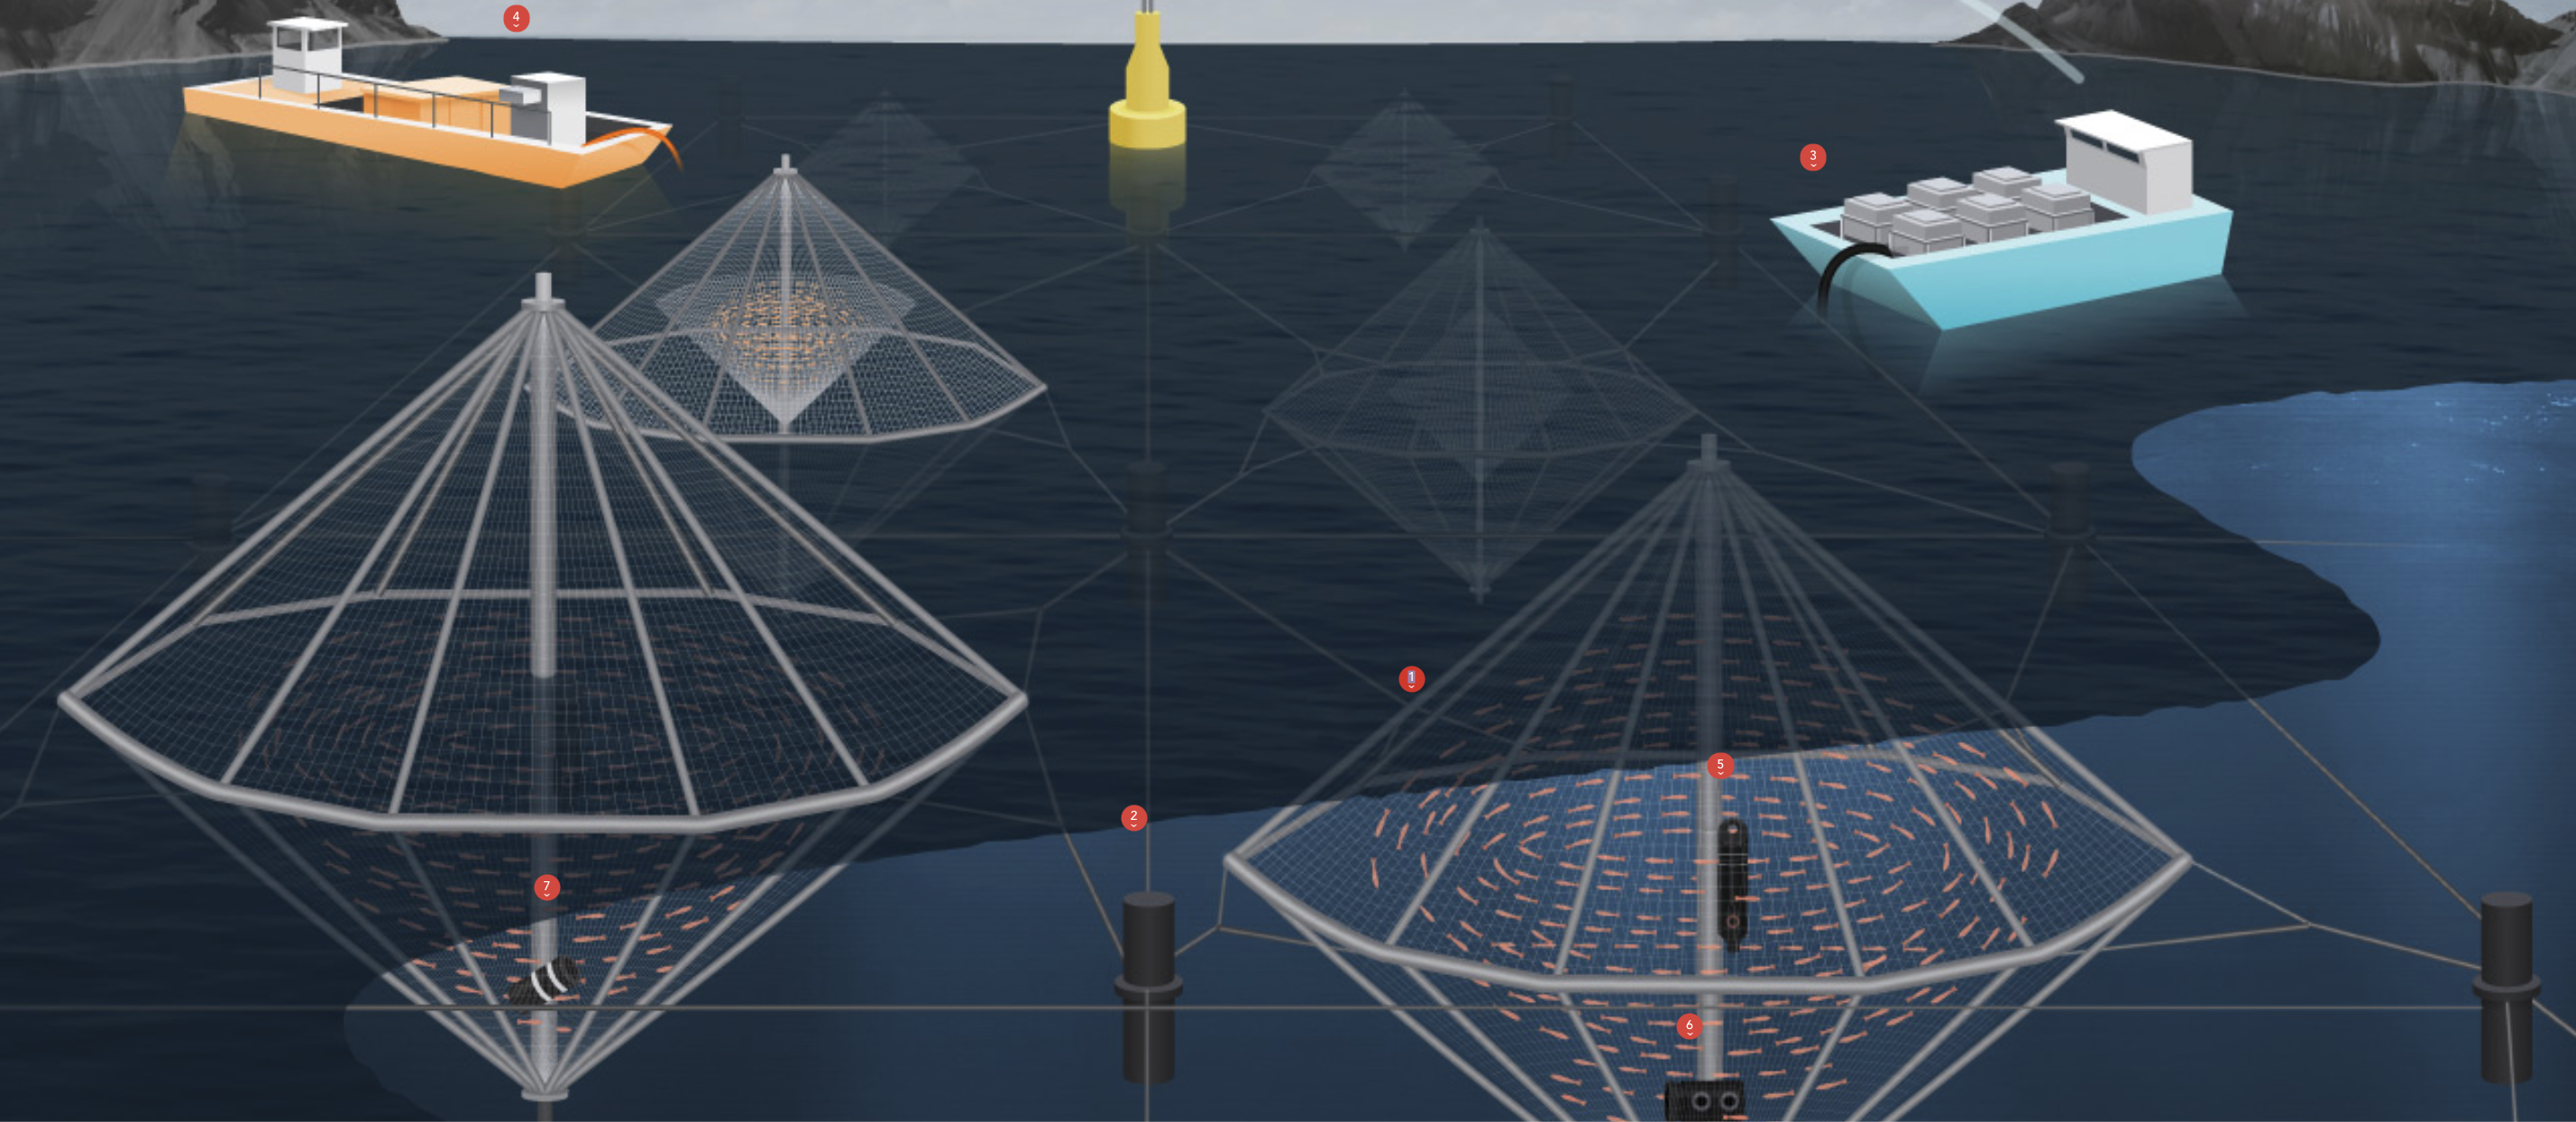
\includegraphics[height=4cm]{images/InnovaSea_1} 
    \caption{\label{fig:InnovaSea_sistema}Distribución de equipos de Innova Sea alrededor de las granjas.}
    \end{center}
\end{figure}


\subsection{Limpieza de redes}
Empresas como Autobots, Watbots o Remora robotics desarrollan robots submarinos con instrumentos que quitan todo material en la red. Los 3 ofrecen una limpieza autónoma,  Watbots y Remora pueden detectar obstáculos y esquivarlos, y Watbots también detecta huecos \cite{Watbots}. Cabe resaltar que estos robots solo poseen un diseño para limpieza de redes, sin la capacidad de ser modular. Asimismo, las empresas se enfocan en realizar servicios en las redes, mas no en las demás partes de la granja. Por este motivo no se le puede agregar una garra para arreglar el hueco, o una cámara para observar el comportamiento del pescado. 


% \cite{Reumann2012}.
%
% \begin{equation}
%   \label{eq:1}
%   a+b=\sqrt{\frac{4}{3}},
% \end{equation}
% donde $a$ y $b$ son escalares.

\section{Métodos de visión computacional}
Los métodos encontrados se basaron de documentos publicados de investigación, ya que las empresas no especifican el software que utilizan. Dado que el objetivo de esta investigación está relacionada con visión computacional, se han encontrado distintos métodos para cada parámetro por detectar en las redes. Estos se dividen en 2: detección de huecos y estimación de suciedad.

\subsection{Detección de huecos}



\subsection{Estimación de suciedad}

\section{Simuladores de sistemas mecatrónicos}

% Entre las causas se pueden considerar la falta de tiempo asignado al taller,
% las limitaciones en cuanto a laboratorios, el poco personal, la falta de una
% correcta selección de los contenidos, así como, una calificación que asegure el
% cumplimiento de los objetivos. Un ejemplo de cómo poner una figura se muestra en la Fig. \ref{fig:diagram2}, y es importante recordar la relación mostrada en \eqref{eq:1}.


% \begin{figure} 
% \begin{center}
% \begin{tabular}{cc}
% 
\includegraphics[height=3cm]{images/logo_utec.png} &
% 
\includegraphics[height=2cm]{images/logo_utec.png} \\
% (a) & (b)
% \end{tabular}
% \caption{\label{fig:diagram2} . (a) Logo en tamaño de 3 centímetros. (b) Logo en tamaño de 2 centímetros.}
% \end{center}
% \end{figure}

% \begin{table}[H]
%     \centering
%     \begin{tabular}{c|c}
%         Tiempo($s$) & Distancia($m$) \\
%         \hline
%         10 & 23 \\
%         20 & 33 \\
%         30 & 43 \\
%         40 & 53 \\
%     \end{tabular}
%     \caption{Tiempos versus distancia.}
%     \label{tab:tiempo_versus_distancia}
% \end{table}